% =====================================================================
%  Deliverable 4 — Generative Artificial Intelligence (580694)
%  Universidad de Concepción · 30 de noviembre de 2026
%  Joaquín Sepúlveda · Renato Saavedra · Lucas Saldivia
%
%  UNA PÁGINA, VERTICAL, compilado desde LaTeX. Overleaf → pdfLaTeX.
%  Las cifras de la prueba sellada salen de scripts/analisis_d4.py sobre
%  resultados/prueba_d4/. Lo que falta está marcado con \PEND{...}.
%  Las curvas: curvas_d4.png (copia de entrenamiento/curvas.png del zip).
% =====================================================================
\documentclass[9pt,a4paper]{extarticle}

\usepackage[T1]{fontenc}
\usepackage[utf8]{inputenc}
\usepackage[spanish,es-noquoting]{babel}
\shorthandoff{"}
\usepackage{libertine}
\usepackage[scaled=0.80]{beramono}
\usepackage{microtype}
\usepackage[margin=8mm]{geometry}
\usepackage{multicol}
\usepackage{xcolor}
\usepackage{booktabs}
\usepackage{tikz}
\usepackage{array}
\usepackage{colortbl}
\usepackage{graphicx}
\usetikzlibrary{arrows.meta,positioning,fit,calc}
\usepackage[hidelinks]{hyperref}
\urlstyle{tt}

\definecolor{tinta}{HTML}{12191A}
\definecolor{acento}{HTML}{B8501C}
\definecolor{verde}{HTML}{146B5F}
\definecolor{ambar}{HTML}{C08A24}
\definecolor{gris}{HTML}{5A6A6B}
\definecolor{fondo}{HTML}{EDF1F0}
\definecolor{linea}{HTML}{C8D4D1}
\definecolor{ajuste}{HTML}{FBE7D6}

\color{tinta}
\pagestyle{empty}
\setlength{\columnsep}{5mm}
\setlength{\multicolsep}{0pt}
\setlength{\parindent}{0pt}
\setlength{\parskip}{0.5mm plus 1mm}
\renewcommand{\arraystretch}{0.93}
\setlength{\tabcolsep}{3.2pt}

\newcommand{\seccion}[1]{\vspace{0.6mm}{\bfseries\footnotesize\color{acento}\MakeUppercase{#1}}\par\nobreak\vspace{0.4mm}\nobreak}
\newcommand{\q}{\textquotedbl}
\newcommand{\cod}[1]{{\ttfamily\small #1}}
\newcommand{\PEND}[1]{{\color{red}\bfseries[#1]}}
\newcommand{\destaque}[1]{%
  \begingroup\setlength{\fboxsep}{2.0mm}%
  \colorbox{fondo}{\parbox{\dimexpr\columnwidth-4.0mm\relax}{#1}}%
  \endgroup\par}

\begin{document}
\raggedright

% ---------------------------------------------------------------- cabecera
{\Large\bfseries \PEND{título con el resultado principal: el Intérprete ajustado con QLoRA ... contra ... del D3 en 239 casos sellados}}\\[0.8mm]
{\footnotesize\color{gris}%
\textbf{Deliverable 4} · Generative Artificial Intelligence (580694) · Universidad de Concepción · 30 de noviembre de 2026\\
\textbf{Grupo 3:} Joaquín Sepúlveda · Renato Saavedra · Lucas Saldivia \quad\textbullet\quad
\textbf{Base:} \cod{microsoft/Phi-3.5-mini-instruct}, 3,8B, NF4, T4 de Colab\\
\textbf{Repositorio:} \href{https://github.com/Luquitas02/genai-inscripcion-ramos}{\cod{github.com/Luquitas02/genai-inscripcion-ramos}} \quad\textbullet\quad
\textbf{Adaptador:} {\small\url{https://huggingface.co/Lss02/phi35-mini-interprete-inscripcion-lora}} (revisión \texttt{99262ad}) \quad\textbullet\quad
\textbf{Video:} \PEND{link}}

\vspace{1mm}
{\color{linea}\rule{\textwidth}{0.4pt}}
\vspace{0.5mm}

\begin{multicols}{2}

% ================================================================ COLUMNA 1
\seccion{Tarea, falla y continuidad}

{\footnotesize
La tarea y el criterio son los del D1 al D3. Dado el historial de un estudiante y una pregunta
en prosa, el sistema decide si puede inscribir el ramo y cita la regla. Un caso es correcto si
acierta decisión y regla (acierto conjunto). La falla del D1 era leer la pregunta. E1 fue no
representar que un ramo se cursa \q ahora\q, y E2 depender de que la pregunta nombre bien el
ramo. El D2 dejó las reglas en código y el D3 repartió la lectura en tres agentes. El D4 ajusta
los pesos del agente que lee, el Intérprete, y deja todo lo demás igual. El sistema del D4 es el
del D3 (v4) con un adaptador LoRA que se activa solo en las llamadas del Intérprete.\par}

\seccion{El grafo de agentes}

\begin{center}
\begin{tikzpicture}[
  font=\scriptsize,
  caja/.style={draw=linea,fill=white,rounded corners=1pt,inner sep=1.3mm,text width=33mm,align=center},
  agente/.style={caja,draw=acento,line width=0.6pt},
  herr/.style={caja,draw=verde,line width=0.6pt,text width=31mm},
  fl/.style={-{Stealth[length=1.5mm]},draw=gris},
  et/.style={font=\tiny,text=gris,align=left},
  node distance=3.8mm]

\node[caja,fill=fondo] (q) {pregunta en prosa};
\node[agente,below=of q,fill=ajuste,line width=1.4pt] (a) {\textbf{A · Intérprete (AJUSTADO)}\\ Phi + adaptador LoRA};
\node[herr,below=6mm of a] (t1) {\textbf{T1 · buscar\_ramo}\\ búsqueda léxica, sin modelo};
\node[agente,below=of t1] (b) {\textbf{B · Resolvedor}\\ Phi base, elige entre 5};
\node[agente,below=of b] (c) {\textbf{C · Verificador}\\ Phi base, contrasta};
\node[herr,below=of c] (t2) {\textbf{T2 · motor de reglas}\\ el código del D2};
\node[caja,fill=fondo,below=of t2] (out) {\textbf{fin} · decisión y regla};
\node[caja,draw=gris,dashed,text width=12mm,right=9mm of a] (fin) {\textbf{fin} sin ramo};
\node[caja,fill=fondo,text width=10mm,right=9mm of t2,yshift=-2.8mm] (hist) {historial};

\draw[fl] (q) -- node[right,et]{texto} (a);
\draw[fl] (a) -- node[right,et]{la mención consultada} (t1);
\draw[fl] (t1) -- node[right,et]{5 candidatos} (b);
\draw[fl] (b) -- node[right,et]{elige: código} (c);
\draw[fl] (c) -- node[right,et]{acepta: código, período} (t2);
\draw[fl] (t2) -- node[right,et]{decisión y regla} (out);
\draw[fl] (hist.west) -- node[below,et]{estados} (hist.west -| t2.east);
\draw[fl,dashed] ($(a.west)+(0,1.2mm)$) -- ++(-9mm,0) |- ($(c.west)+(0,1.2mm)$);
\draw[fl,dashed] ($(a.west)+(-9mm,1.2mm)$) |- ($(b.west)+(0,1.2mm)$);
\node[et,anchor=south,inner sep=0.4mm] at ($(b.west)+(-6mm,1.2mm)$) {otros};
\node[et,anchor=south east,inner sep=0.4mm] at ($(c.west)+(-0.8mm,1.2mm)$) {otros,\\ período};
\draw[fl,dashed] (a) -- node[above,et]{sin\_ramo} (fin);
\draw[fl] (q.east) -- ++(26mm,0) |- node[pos=0.2,left,et,align=right]{pregunta} ($(c.east)+(0,1.2mm)$);
\draw[fl] (b.east) -- ++(4.5mm,0) |- node[pos=0.25,right,et]{busca de nuevo\\ (máx. 2)} (t1.east);
\draw[fl] (c.west) -- ++(-15mm,0) |- node[pos=0.3,left,et,align=right]{rechaza\\ con motivo;\\ máx. 2} (a.west);
\end{tikzpicture}
\end{center}

{\footnotesize\color{gris} Relleno naranjo, el agente ajustado. Los tres agentes corren sobre
un solo Phi cargado una vez. El adaptador se apaga en las llamadas de B y C, que siguen con la
base. Prompts sin cambios, cada uno en \cod{prompts/<agente>.md}.\par}

\seccion{Por qué el Intérprete y por qué fine-tuning}

{\footnotesize
En las trazas del D3 (403 casos), de los 34 errores de prueba 14 eran referencias ambiguas por
construcción (\q gestión\q, \q electiva\q), que ningún agente puede resolver, 8 eran del
Resolvedor y los arregla una regla de una línea, y 11 nacían en el Intérprete, en el período o en
la mención. Con prosa más variada (piloto, 60 casos de desarrollo) el D3 baja a 52 de 60 y el
error está en el Intérprete. Lee \q este segundo semestre\q\ como el próximo y no entiende apodos
como \q evapro\q.

El prompting ya llegó a su límite. El prompt v3 define el período con fechas, trae 4 ejemplos y
pide copiar la frase antes de decidir, y aun así decide al revés con la frase copiada. La v5 y la
v6 corrigieron con prompts y no superaron a la v4. Más ejemplos no caben. Con 40 el prompt mide
4.031 tokens, Phi-3.5 pasa su límite de 4.096 al generar y escribe basura en 20 de 60 casos. Lo
que hay que enseñar es una conducta (leer el período en la frase correcta), y eso es lo que la
Lecture 8 asigna al fine-tuning.\par}

\seccion{Datos de entrenamiento}

{\footnotesize
\begin{tabular}{@{}lrl@{}}
\toprule
bloque & pares & de dónde sale \\
\midrule
prosa variada, 6 estilos & 1.199 & casos del generador, mensaje de Claude \\
plantillas del generador & 150 & el generador del D1 \\
turnos de revisión & 60 & la entrada trae un rechazo de C \\
sin asignatura & 20 & mensaje de Claude, salida \cod{sin\_ramo} \\
\midrule
\textbf{total} & \textbf{1.429} & 1.286 entrenamiento, 143 validación \\
\bottomrule
\end{tabular}\par}

\vspace{0.4mm}
{\footnotesize
\textbf{Etiquetas.} El período, el ramo y los ramos de contexto salen del caso del generador, no
de un modelo. Los mensajes los escribieron 21 subagentes de Claude (Anthropic) con una
instrucción versionada. Cada uno declaró las palabras exactas del ramo y del período, y un script
exigió que estuvieran literalmente en el mensaje (1.260 de 1.260). Un lector automático a ciegas
coincidió con la etiqueta en 1.242 de 1.260. \textbf{Revisión a mano}, 120 pares al azar en dos
muestras de 60, 30 por persona. En la primera, 7 de 60 tenían apodos que un estudiante no usaría,
con la etiqueta bien copiada. En la segunda, 0 de 60 incorrectas y 4 que \q suenan raro pero se
entienden\q. \textbf{Separación de la prueba} (\cod{separacion\_d4.py}). Ningún caso comparte
historial y consulta con uno de prueba, ninguna pregunta es igual ni casi igual (difflib máx.
0,848), y 7,3\,\% de los 6-gramas de la prueba aparecen en el entrenamiento, contra 8,5\,\% dentro
de la propia prueba.\par}

% ================================================================ COLUMNA 2
\columnbreak

\seccion{Entrenamiento}

{\footnotesize
QLoRA (Lecture 8). Base en NF4 congelada, LoRA de rango 16, alpha 32, dropout 0,05 en todas las
capas lineales (25,2 millones de parámetros entrenables, menos del 1\,\% del modelo). Learning rate 2e-4
lineal, 3 pasos de calentamiento, batch 2 por 4 de acumulación, fp16, pérdida solo sobre la
respuesta. 2 épocas, 322 pasos, 114 min en una Tesla T4 de Colab gratuita, 3,6 GB de
memoria. Las dos épocas acertaron 55 de 60 en el piloto y la regla del protocolo desempató por
la pérdida de validación (0,0127 en la primera y 0,0113 en la segunda), así que se publicó la segunda.\par}

\vspace{0.3mm}
\begin{center}
\IfFileExists{curvas_d4.png}{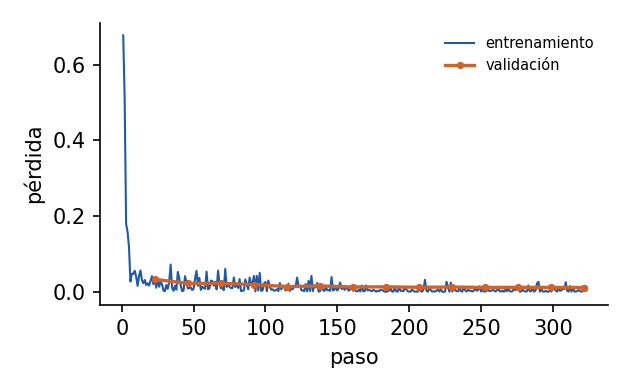
\includegraphics[width=0.86\columnwidth]{curvas_d4.png}}%
{\fbox{\parbox[c][30mm][c]{0.8\columnwidth}{\centering\PEND{curvas de pérdida}}}}
\end{center}

\seccion{Resultados en 239 casos sellados}

{\footnotesize Casos con decisión y regla correctas. Prueba sellada antes de generar los datos
de entrenamiento. Período: la prosa dice cuándo y eso decide la respuesta.\\
\begin{tabular}{@{}lrrrrr@{}}
\toprule
& plantilla & \multicolumn{3}{c}{redactadas (179)} & \\
\cmidrule(lr){3-5}
acierto conjunto & (60) & período act. & período próx. & otras & \textbf{239} \\
\midrule
baseline few-shot (D1)   & \PEND{} & & & & \\
sistema del D2           & & & & & \\
sistema del D3 (v4)      & & & & & \\
\rowcolor{fondo}
\textbf{D4, Intérprete ajustado} & & & & & \\
control: D3 con 27 ejemplos más & & & & & \\
regla fija, sin modelo   & 38 & 26 & 0 & 31 & 95 \\
\bottomrule
\end{tabular}\par}

\vspace{1mm}
\destaque{\footnotesize \PEND{D4 contra D3: gana ..., pierde ..., McNemar exacto p = .... D4 contra el control: ...}}

\vspace{0.4mm}
{\footnotesize
\textbf{El control} es el D3 con el mismo prompt y 27 ejemplos de los datos de entrenamiento,
los que caben bajo 3.600 tokens. Ve en el prompt los datos que el ajuste ve en los pesos.
\PEND{lectura del período del Intérprete, estricto, lo que no se rompió}\par}

\seccion{Caso de falla}

{\footnotesize \PEND{primer redactado, en orden de id, que el D4 falla; traza en el repositorio}\par}

\seccion{Cómo se midió}

{\footnotesize
\textbf{Prueba.} 239 casos nuevos: 60 de plantilla y 179 escritos por subagentes de Claude que
no vieron el sistema ni los datos de entrenamiento. Un lector automático a ciegas comparó cada
mensaje con su etiqueta y uno de nosotros leyó los 3 desacuerdos y 30 acuerdos al azar. sha256
en \cod{SELLO.txt} desde el 24 de noviembre. \textbf{Protocolo.} \cod{PROTOCOLO\_D4.md} quedó en
el repositorio antes de entrenar, con la elección de época, el control, las filas y el análisis.
La prueba se corrió una vez, con el adaptador bajado de Hugging Face en la revisión publicada y
su sha256 comprobado. Cada mensaje entre agentes está en las trazas con el hash de su prompt.\par}

\seccion{Límites declarados}

{\footnotesize
\textbf{Mismo redactor.} Claude escribió la prosa de entrenamiento y la de prueba, con casos e
instrucciones distintos. \textbf{Oferta semestral.} El sistema nunca modeló en qué semestre se
dicta cada ramo. Con la oferta real, 52 de las 129 respuestas afirmativas de la prueba serían
\q no se dicta\q. \textbf{Etiquetas.} Las genera el mismo motor de reglas que usa T2.\par}

\end{multicols}
\end{document}
